\chapter{Desenvolvimento do projeto}
\label{chap:metod}
Nesta seção será descrito o procedimento utilizado para construção inicial do robô Walker, incluindo as fases conceitual e design.  Será apresentado a ideação do projeto, especificações e as funcionalidades.

\section{Ideação}
%escrever oq sera apresentado

\subsection{Arquitetura Geral}
 A arquitetura geral, apresentada na Figura \ref{fig:Arquitetura geral}, relaciona de modo geral a interface do usuário, com a central de gerenciamento do sistema e com a interface com hardware. Neste contexto, a interface do usuário representa o contato direto com o usuário por meio de um botão \textit{on/off}, um \textit{joystick} e por acesso remoto, através de um computador devidamente conectado.

 \begin{figure} [h!]	
    \centering

    \caption{Arquitetura Geral}
    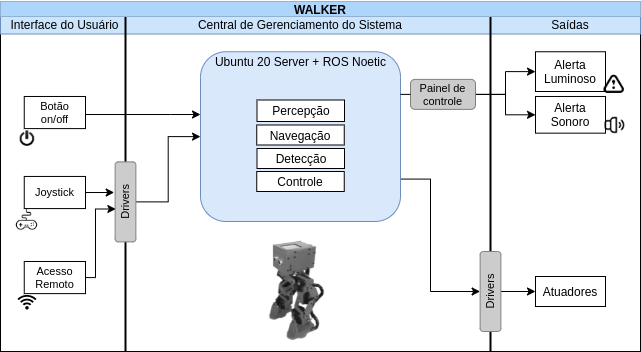
\includegraphics[width=0.8\textwidth]{general_architecture}
    \caption*{Fonte: Autoria própria.}
    \label{fig:Arquitetura geral}
\end{figure}	

Para a central de gerenciamento do sistema utilizou-se o sistema operacional \textit{Ubuntu} 20.04 junto ao framework de robótica ROS \textit{Noetic}. Neste cojunto se encontram as principais funcionalidades do robô: percepção, navegação, detecção e controle. Por fim, no conjunto de saídas estão os atuadores e os alertas sonoro e luminoso.

\subsection{Requisitos técnicos}

%desdobramento da função qualidade
\subsection{Quality Function Deployment}
\textit{Quality Function Deployment} é uma ferramenta de qualidade que auxilia na conversão das demandas do cliente em características de qualidade do produto. Dessa forma, no primeiro ciclo do QFD foram analisados os requisistos do cliente e os requisitos técnicos necessários, sinalizando os pontos mais importantes e as relações entre estes. O resultado foi exposto na \ref{fig:QFD}

\begin{figure} [h!]	
    \centering
    \caption{ Primeiro ciclo QFD}
    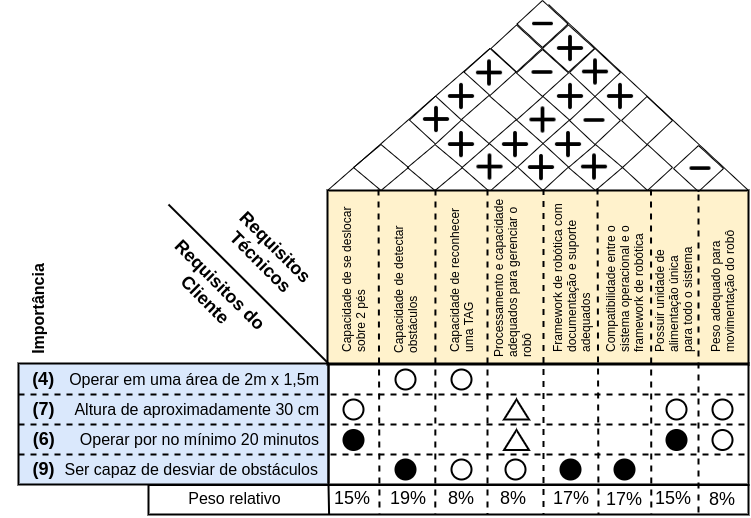
\includegraphics[width=0.8\textwidth]{Figures/QFD}
    \caption*{Fonte: Autoria própria.}
    \label{fig:QFD}
\end{figure}
 Através do QFD foi possível observar 

% %--------- NEW SECTION ----------------------
% \section{Interface do Usuário}
% \label{sec:ui}
% \lipsum[1]

% %--------- NEW SECTION ----------------------
% \section{Simulação do sistema}
% \label{sec:sim}
% \lipsum[2-4]

